\subsection{Functional Requirements}
We define the high-level functional requirements for the router here. For a 
more detailed description refer to \autoref{sec:packet_processing}.

\paragraph{Termination (bounded execution)}
Processing any packet is guaranteed to halt, i.e., no more that N 
instructions are executed per packet.

\paragraph{Crash freedom}
The code is guaranteed to never execute any instruction that would cause it 
to terminate abnormally (for a meaningful definition of abnormally).

\paragraph{Functional correctness}
The code implements all the functionality defined in the specification and 
performs it correctly. This includes but is not limited to
\begin{itemize}
	\item how incoming packets get processed (e.g., a router must not 
	change the payload of a packet, a router must verify the current opaque 
	field etc.)
	\item how incoming packets can change the state of the router
	\item what kind of modifications to the packet header are allowed and 
	correct for the different packet types
\end{itemize}

\subsection{Security Requirements}
\paragraph{Non-interference}
Basically this means that no sensitive data (e.g., installed 
encryption/signature keys) gets leaked in any kind. This captures 
\begin{itemize}
	\item an explicit data flow, where the secret gets leaked explicitly, e.g., 
	by sending it out of the router or writing it to an unprotected part of the 
	memory.
	\item an implicit data flow, where the secret gets leaked implicitly, e.g., 
	through computation that is dependent on the value of the secret.
\end{itemize}
Note, that noninterference is a term that is only applicable to deterministic 
programs.
Especially, it does not apply to multi-threaded executions, since the 
scheduler is a source of nondeterminism. For that we have to look a 
probabilistic noninterference, which is a much harder property to prove.

\paragraph{‘Bounded’ I/O}
For each packet received, the router sends out at most one packet to the 
intended next hop or drops the packet, if that is the correct behavior (e.g., 
if OF verification fails)

\paragraph{No pro-active behavior}
The router must not perform any operation that was not initially triggered by 
a ‘PacketIn’ event. Exceptions to this rule are:
\begin{enumerate}
	\item Periodically sending a keep-alive message to the peering router
\end{enumerate}

\subsection{Packet processing}\label{sec:packet_processing}
In this section we define how each packet type must be handled by the 
router. \autoref{fig:scion_packet} shows the layout of a generic SCION packet. 
Most forwarding decisions involve the path - a list of opaque fields containing 
the AS-local routing decision - and the two pointers \currof and 
\curriof. \currof always points to the current opaque field that needs to be 
processed by the router, whereas \curriof points to the info opaque field of 
the current path segment.

\begin{figure}
\centering
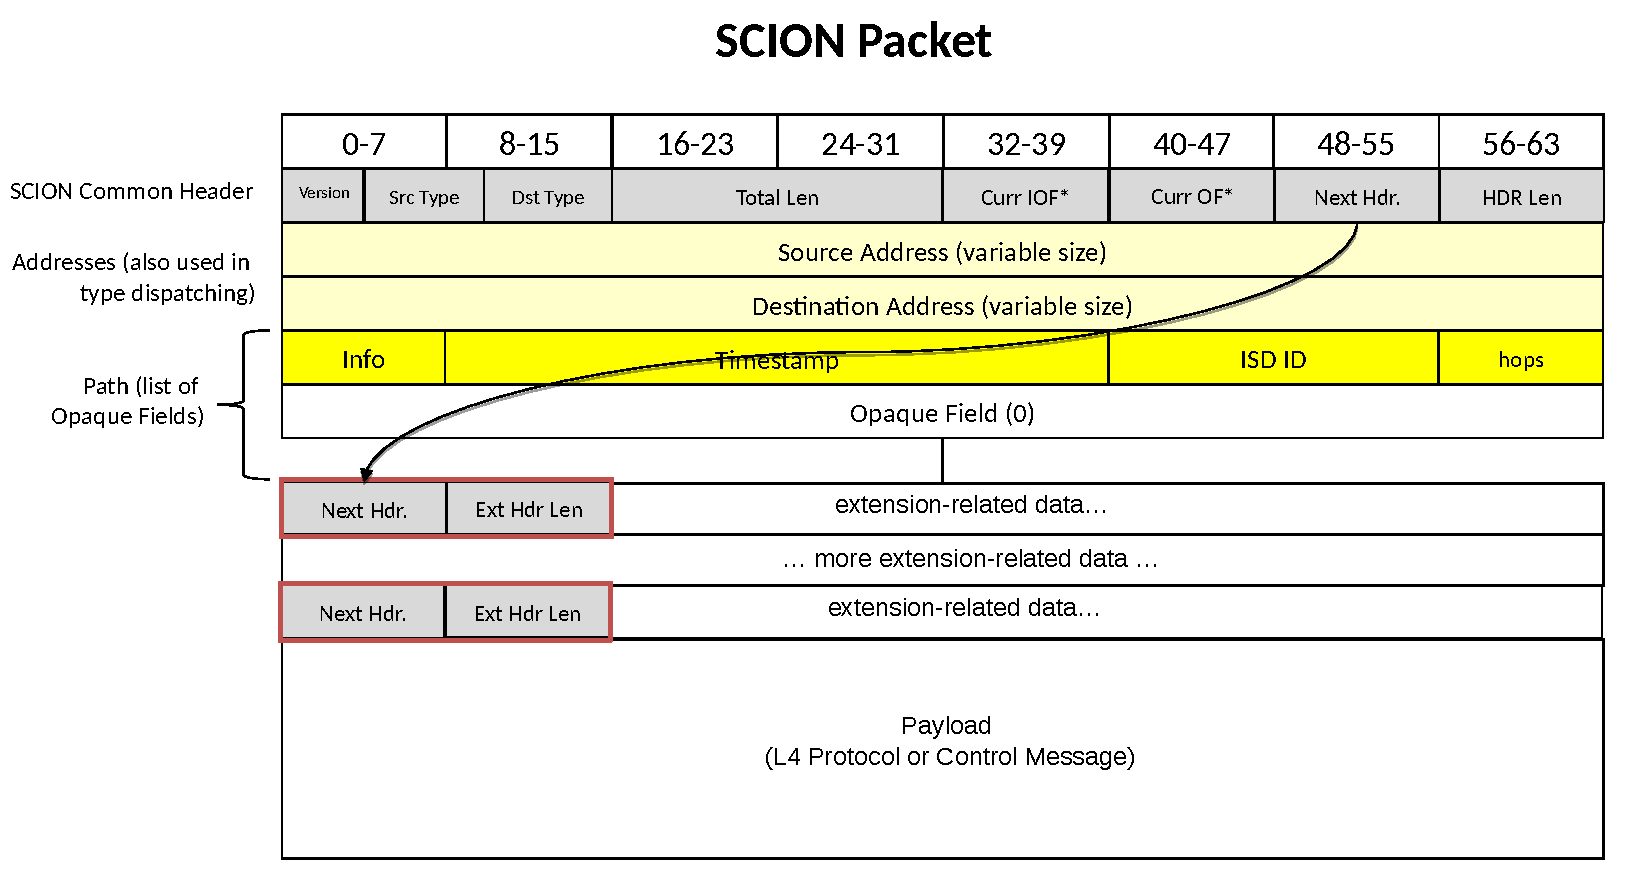
\includegraphics[width=\textwidth]{figs/scion_packet}
\caption{Generic SCION Packet}
\label{fig:scion_packet}
\end{figure}

\subsubsection{Data Packets}\label{sec:data_packet_processing}
Data packets always carry a complete end-to-end path in the header. We 
distinguish between three types of end-to-end paths.

\paragraph{Core Path}
A core path is a (non-shortcut) path through the ISD core. 
\autoref{fig:core_path} shows the sequence of opaque fields for a core path. 
Fields highlighted in blue denote \textit{crossover} points and the 
corresponding opaque fields have this field set.
\begin{figure}
\centering
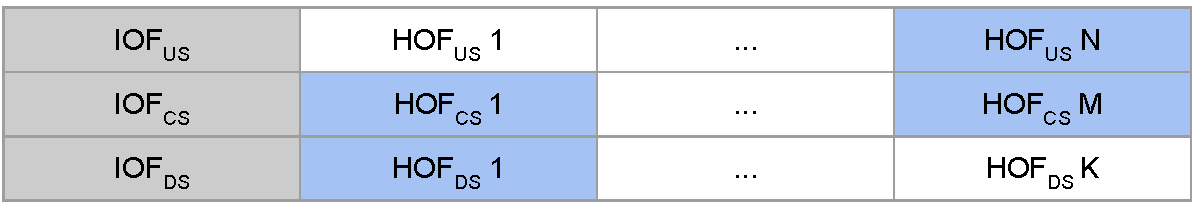
\includegraphics[width=0.8\textwidth]{figs/core_path}
\caption{Core Path}
\label{fig:core_path}
\end{figure}

\paragraph{Peer Path}
A peer path is an end-to-end path that involves a peering link between two 
ASes. \autoref{fig:peer_path} shows the sequence of opaque fields for a peer 
path. HOF\tus{US} N and HOF\tus{DS} 1 as well as AUTH\tus{US} and AUTH\tus{DS} 
are not used for actual routing but to authenticate the peering link. The 
authentication chain for the up-segment looks like this:
\[
	\text{AUTH\_OF}_\text{US} \quad \xrightarrow{auth}\quad 
	\text{HOF}_\text{US} \, \text{N} \quad \xrightarrow{auth} \quad 
	\text{PEER\_OF}_\text{US}
\]

\begin{figure}
	\centering
	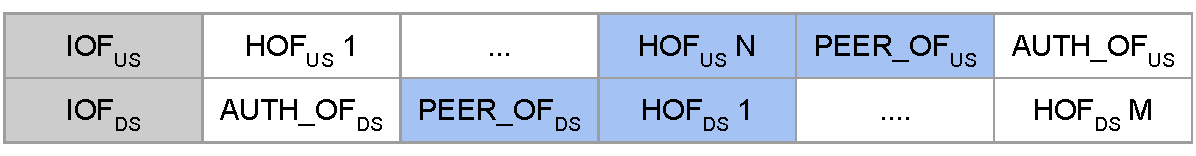
\includegraphics[width=0.8\textwidth]{figs/peer_path}
	\caption{Peer Path}
	\label{fig:peer_path}
\end{figure}

\paragraph{Shortcut Path}
A shortcut path is a path where the up- and down-segment intersect at a 
non-core AS. This is the case of a shortcut where up-segment and 
down-segment meet before entering the ISD core. \autoref{fig:shortcut_path} 
shows the sequence of opaque fields for a shortcut path. AUTH\_OF\tus{\{US, 
DS\}} are used to authenticate HOF\tus{US} N, respectively HOF\tus{DS} 1. 
HOF\tus{US} N and HOF\tus{DS} 1 together define the shortcut and are combined 
for the forwarding decision.

The special case when the source's up-segment contains the destination AS is 
treated as a shortcut path.\newline

\begin{figure}
	\centering
	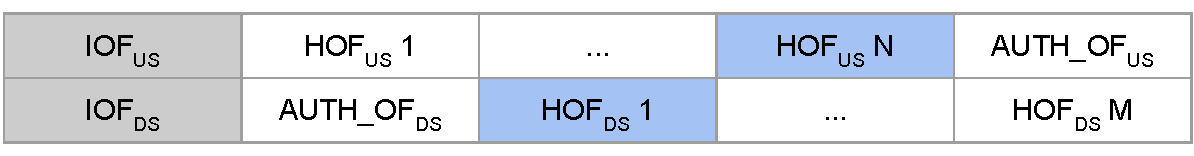
\includegraphics[width=0.8\textwidth]{figs/shortcut_path}
	\caption{Shortcut Path}
	\label{fig:shortcut_path}
\end{figure}


\noindent
In the following we describe the algorithms for data packet processing. We 
distinguish between cases for ingress and egress routers as well as for the 
different types of paths. The different path types only influence the 
processing when switching from one path segment to the next. Additionally, the 
\verb|ingress_normal_foward| and \verb|egress_normal_forward| cases cover the 
processing of an opaque field that is not the end of a segment, independent of 
the type of the path.

The following invariants have to hold and be preserved by the packet processing 
code:
\begin{enumerate}
\item On 'PacketIn' \currof always points to the opaque field that needs to be 
verified and is used to make the routing decision.
\item \curriof always points to the path segment that \currof belongs to.
\item All routers verify the MAC of the OF that \currof points to.
\item Only ingress router terminate paths, i.e., forward the packet to a 
destination within the local AS.
\end{enumerate}
\begin{algorithm}
\caption{ingress\_normal\_forward}
\begin{algorithmic}
\Require{
	\item pkt received on inter-domain interface
	\item \anot pkt.curr\_of.is\_xovr\_point()
}
\Ensure{
	\item pkt.curr\_of = \aold{pkt.curr\_of}
	\item pkt.curr\_iof = \aold{pkt.curr\_iof}\\	
}
\Procedure{ingress\_normal\_forward}{pkt, if2addr}
\If{pkt.is\_on\_up\_path()}
	\State{fwd\_if := pkt.curr\_of.ingress\_if}
	\State{prev\_of := pkt.get\_relative\_of(1)}
\Else
	\State{fwd\_if := pkt.curr\_of.egress\_if}
	\State{prev\_of := pkt.get\_relative\_of(-1)}
\EndIf
\If{\anot verify(pkt.curr\_of, prev\_of, pkt.curr\_iof.ts)}
	\State{\textit{drop pkt}}
\EndIf
\If{fwd\_if == 0 \aand pkt.is\_last\_hop()}
	\State{\Call{send}{pkt, pkt.dst\_addr}}
\Else
	\State{\Call{send}{pkt, if2addr[fwd\_if]}}
\EndIf
\EndProcedure
\end{algorithmic} 
\end{algorithm}

\begin{algorithm}
\caption{egress\_normal\_forward}
\begin{algorithmic}
\Require{
	\item pkt received on intra-domain interface
	\item \anot pkt.curr\_of.is\_xovr\_point()
}
\Ensure{
	\item pkt.curr\_of = \aold{pkt.curr\_of} + 8
	\item pkt.curr\_iof = \aold{pkt.curr\_iof}	\\
}
\Procedure{egress\_normal\_forward}{pkt, next\_hop}
\If{pkt.is\_on\_up\_path()}
	\State{prev\_of := pkt.get\_relative\_of(1)}
\Else
	\State{prev\_of := pkt.get\_relative\_of(-1)}
\EndIf
\If{\anot verify(pkt.curr\_of, prev\_of, pkt.curr\_iof.ts)}
	\State{\textit{drop pkt}}
\EndIf
\State{pkt.curr\_of := pkt.curr\_of + 8}
\State{\Call{send}{pkt, next\_hop}}
\EndProcedure
\end{algorithmic} 
\end{algorithm}

\begin{algorithm}
\caption{ingress\_shortcut\_xovr}
\begin{algorithmic}
\Require{
	\item pkt received on inter-domain interface
	\item pkt.curr\_iof.info == SHORTCUT\_PATH
	\item pkt.curr\_of.is\_xovr\_point() (HOF\tus{US} N)
	\item pkt.is\_on\_up\_path()
}
\Ensure{
	\item pkt.curr\_of = \aold{pkt.curr\_of} + 32 (HOF\tus{DS} 1)
	\item pkt.curr\_iof = \aold{pkt.curr\_of} + 16 (IOF\tus{DS})\\	
}
\Procedure{ingress\_shortcut\_xovr}{pkt, if2addr}
\If{\anot verify(pkt.curr\_of, pkt.get\_relative\_of(1), pkt.curr\_iof.ts)}
	\State{\textit{drop pkt}}
\EndIf
\State{pkt.curr\_iof := pkt.curr\_of + 16}
\State{pkt.curr\_of := pkt.curr\_of + 32}
\If{pkt.curr\_of.egress\_if == 0 \aand pkt.is\_last\_hop()}
	\If{\anot verify(pkt.curr\_of, pkt.get\_relative\_of(-1), pkt.curr\_iof.ts)}
		\State{\textit{drop pkt}}
	\EndIf
	\State{\Call{send}{pkt, pkt.dst\_addr}}
\Else
	\State{\Call{send}{pkt, if2addr[pkt.curr\_of.egress\_if]}}
\EndIf
\EndProcedure
\end{algorithmic} 
\end{algorithm}

\begin{algorithm}
\caption{egress\_shortcut\_xovr}
\begin{algorithmic}
\Require{
	\item pkt received on intra-domain interface
	\item pkt.curr\_iof.info == SHORTCUT\_PATH
	\item pkt.curr\_of.is\_xovr\_point() (HOF\tus{DS} 1)
	\item \anot pkt.is\_on\_up\_path()\\
}
\Procedure{egress\_shortcut\_xovr}{pkt, next\_hop}
\State{\Call{egress\_normal\_forward}{pkt, next\_hop}}
\EndProcedure
\end{algorithmic} 
\end{algorithm}

\begin{algorithm}
\caption{ingress\_peer\_xovr}
\begin{algorithmic}
\Require{
	\item pkt received on inter-domain interface
	\item pkt.curr\_iof.info == PEER\_PATH
	\item pkt.curr\_of.is\_xovr\_point() (HOF\_OF\tus{US} N)
}
\Ensure{
	\item pkt.curr\_of = \aold{pkt.curr\_of} + 8 (PEER\_OF\tus{US})
	\item pkt.curr\_iof = \aold{pkt.curr\_iof}\\
}
\Procedure{ingress\_peer\_xovr}{pkt, if2addr}
\If{pkt.is\_on\_up\_path()}
	\If{\anot verify(pkt.curr\_of, pkt.get\_relative\_of(2), pkt.curr\_iof.ts)}
		\State{\textit{drop pkt}}
	\EndIf
	\State{pkt.curr\_of := pkt.curr\_of + 8}
	\State{\Call{send}{pkt, if2addr[pkt.curr\_of.ingress\_if]}}
\Else
	\If{\anot verify(pkt.curr\_of, pkt.get\_relative\_of(1), pkt.curr\_iof.ts)}
		\State{\textit{drop pkt}}
	\EndIf
	\State{pkt.curr\_of := pkt.curr\_of + 8}
	\If{pkt.is\_last\_hop()}
		\State{\Call{send}{pkt, pkt.dst\_addr}}
	\Else
		\State{\Call{send}{pkt, if2addr[pkt.curr\_of.egress\_if]}}
	\EndIf
\EndIf
\EndProcedure
\end{algorithmic} 
\end{algorithm}

\begin{algorithm}
\caption{egress\_peer\_xovr}
\begin{algorithmic}
\Require{
	\item pkt received on intra-domain interface
	\item pkt.curr\_iof.info == PEER\_PATH
	\item pkt.curr\_of.is\_xovr\_point() (PEER\_OF\tus{US})
}
\Ensure{
	\item pkt.is\_on\_up\_path() $\implies$ pkt.curr\_of = \aold{pkt.curr\_of} 
	+ 32 (HOF\tus{DS} 1)
	\item pkt.is\_on\_up\_path() $\implies$ pkt.curr\_iof = \aold{pkt.curr\_of} 
		+ 16 (IOF\tus{DS})
	\item \anot pkt.is\_on\_up\_path() $\implies$ pkt.curr\_of = 
	\aold{pkt.curr\_of} + 8 
	\item \anot pkt.is\_on\_up\_path() $\implies$ pkt.curr\_iof = 
	\aold{pkt.curr\_iof}\\
}
\Procedure{egress\_peer\_xovr}{pkt, next\_hop}
\If{pkt.is\_on\_up\_path()}
	\If{\anot verify(pkt.curr\_of, pkt.get\_relative\_of(-1), pkt.curr\_iof.ts)}
		\State{\textit{drop pkt}}
	\EndIf
	\State{pkt.curr\_iof := pkt.curr\_of + 16}
	\State{pkt.curr\_of := pkt.curr\_of + 32}
\Else
	\If{\anot verify(pkt.curr\_of, pkt.get\_relative\_of(-2), pkt.curr\_iof.ts)}
		\State{\textit{drop pkt}}
	\EndIf
	\State{pkt.curr\_of := pkt.curr\_of + 8}
\EndIf
\State{\Call{send}{pkt, next\_hop}}
\EndProcedure
\end{algorithmic} 
\end{algorithm}

\begin{algorithm}
\caption{ingress\_core\_xovr}
\begin{algorithmic}
\Require{
	\item pkt received on inter-domain interface
	\item pkt.curr\_iof.info == CORE\_PATH
	\item pkt.curr\_of.is\_xovr\_point()
}
\Ensure{
	\item \anot \aold{pkt.is\_last\_hop()} $\implies$ pkt.curr\_of = 
	\aold{pkt.curr\_of} + 16
	\item \anot \aold{pkt.is\_last\_hop()} $\implies$ pkt.curr\_iof = 
	\aold{pkt.curr\_of} + 8 \\	
}
\Procedure{ingress\_core\_xovr}{pkt, if2addr}
\If{pkt.is\_on\_up\_path()}
	\State{prev\_of := None}
\Else
	\State{prev\_of := pkt.get\_relative\_of(-1)}
\EndIf
\If{\anot verify(pkt.curr\_of, prev\_of, pkt.curr\_iof.ts)}
	\State{\textit{drop pkt}}
\EndIf
\If{pkt.is\_last\_hop()}
	\State{\Call{send}{pkt, pkt.dst\_addr}}
\Else
	\State{pkt.curr\_iof := pkt.curr\_of + 8}
	\State{pkt.curr\_of := pkt.curr\_of + 16}
	\If{pkt.is\_on\_up\_path()}
		\State{\Call{send}{pkt, if2addr[pkt.curr\_of.ingress\_if]}}
	\Else
		\State{\Call{send}{pkt, if2addr[pkt.curr\_of.egress\_if]}}
	\EndIf
\EndIf
\EndProcedure
\end{algorithmic} 
\end{algorithm}

\begin{algorithm}
\caption{egress\_core\_xovr}
\begin{algorithmic}
\Require{
	\item pkt received on intra-domain interface
	\item pkt.curr\_iof.info == CORE\_PATH
	\item pkt.curr\_of.is\_xovr\_point()
}
\Ensure{
	\item pkt.curr\_of = \aold{pkt.curr\_of} + 8	
}
\Procedure{egress\_core\_xovr}{pkt, next\_hop}
\If{\anot pkt.is\_on\_up\_path()}
	\State{prev\_of := None}
\Else
	\State{prev\_of := pkt.get\_relative\_of(1)}
\EndIf
\If{\anot verify(pkt.curr\_of, prev\_of, pkt.curr\_iof.ts)}
	\State{\textit{drop pkt}}
\EndIf
\State{pkt.curr\_of := pkt.curr\_of + 8}
\State{\Call{send}{pkt, next\_hop}}
\EndProcedure
\end{algorithmic} 
\end{algorithm}

\clearpage
\subsubsection{Control Packets}
With the exception of path management packets, control packets do not contain a 
path in their packet header. In general, control packets are either forwarded 
to the corresponding infrastructure server\footnote{Beacon Servers, Path 
Servers and Certificate Servers} (on the ingress router) or passed on to the 
neighboring AS (on the egress router). The infrastructure servers then decide 
to which egress router a control packets needs to get forwarded to.

\paragraph{Path Construction Beacons}
\autoref{alg:process_pcb} shows the algorithm to process a PCB.
\begin{algorithm}
\caption{process\_pcb}
\label{alg:process_pcb}
\begin{algorithmic}
\Require{
	\item pkt.type = PATH\_CONSTRUCTION\_BEACON
}
\Procedure{process\_pcb}{pkt, next\_hop}
\If{pkt.src\_addr == BS.addr}
	\State{\Call{send}{pkt, next\_hop}}
\Else
	\State{\Call{send}{pkt, BS.addr}}
\EndIf
\EndProcedure
\end{algorithmic} 
\end{algorithm}

\paragraph{Certificate and TRC Packets}
\autoref{alg:process_cert} shows the algorithm to process a packet coming from 
or destined to a certificate server.
\begin{algorithm}
\caption{process\_cert\_packet}
\label{alg:process_cert}
\begin{algorithmic}
\Require{
	\item pkt.type \ain \{CERT\_REQ, CERT\_REP, TRC\_REQ, TRC\_REP\}
}
\Procedure{process\_cert\_packet}{pkt, next\_hop}
\If{pkt.src\_addr == CS.addr}
	\State{\Call{send}{pkt, next\_hop}}
\Else
	\State{\Call{send}{pkt, CS.addr}}
\EndIf
\EndProcedure
\end{algorithmic} 
\end{algorithm}

\paragraph{Path Management Packets}
Path management packets are the only type of control packets that contain a 
path in the header. Thus, handling a path management packet is already covered 
by \autoref{sec:data_packet_processing}.

\paragraph{Keep-Alive Packets}
Keep-alive packets are periodically sent by the router to a neighboring router 
to indicate that the link and router are still up and running. Keep-alive 
packets must be forwarded to the local beacon server which keeps track about 
router and link statuses.

\begin{algorithm}
\caption{sync\_interface}
\label{alg:sync_interface}
\begin{algorithmic}
\Procedure{sync\_interface}{if\_id, next\_hop}
\While{True}
	\State{pkt := KeepAlivePkt(if\_id)}
	\State{\Call{send}{pkt, next\_hop}}
	\State{\Call{sleep}{KEEP\_ALIVE\_INTERVAL}}
\EndWhile
\EndProcedure
\end{algorithmic} 
\end{algorithm}

\begin{algorithm}
\caption{process\_keep\_alive\_packet}
\label{alg:process_keep_alive_packet}
\begin{algorithmic}
\Require{
	\item pkt.type == KEEP\_ALIVE
}
\Procedure{process\_keep\_alive\_packet}{pkt}
\State{\Call{send}{pkt, BS.addr}}
\EndProcedure
\end{algorithmic} 
\end{algorithm}
